\chapter{Conception}
\section{Purpose of the chapter}
The purpose of this chapter is to present the conception of a virtual counter system for the Algerian National Social Security Fund (CNAS). This chapter will provide a detailed explanation of the system design and architecture, database design, as well as the different diagrams and models used during the conception phase. The virtual counter system aims to improve the current management system used by CNAS by providing users with a more efficient and user-friendly way to gather necessary information and book appointments.
\section {Overview of the topics covered}
This chapter focuses on the conception of the virtual counter system for CNAS. It includes the analysis and design of the system, from the identification of user requirements to the development of the system architecture and database design. The chapter also includes the presentation of the different diagrams that were created, such as the use case diagram, class diagram.
The aim of this chapter is to provide a comprehensive understanding of the virtual counter system, its components, and its functionalities.

\section{System design and architecture}
The system design and architecture of a virtual counter is a crucial aspect in developing a successful web application. It involves designing the components of the system and specifying how they interact with each other to achieve the desired functionality. In the case of a virtual counter for CNAS, the system design and architecture must take into account the different types of users, such as clients and agents, and the various tasks they need to perform. It must also ensure that the application is secure and reliable, with measures in place to protect user data and prevent unauthorized access. The system design and architecture will involve selecting suitable technologies and frameworks, such as Laravel and VueJs, and designing a database schema to store and retrieve data efficiently. Overall, a well-designed system architecture will contribute to the effectiveness and efficiency of the virtual counter and improve the user experience for both clients and agents.

\subsection{Description of the overall system architecture}
The overall system architecture of the virtual counter for CNAS is designed to be a web-based application with a client-server architecture. The client-side will be a user-friendly interface, developed using Vue.js framework, that allows users to interact with the system and perform different tasks, such as filling in a questionnaire that will generate a checklist of required documents, booking appointments, and checking their status. On the other hand, the server-side of the application will handle all the processing and data storage. It will be developed using the Laravel framework, which is a powerful and reliable PHP web application framework that enables rapid application development with a robust and scalable codebase. The application will also use a MariaDB database to store all the necessary data, such as user information, appointment schedules, and queue status. The overall system architecture is designed to be modular and scalable, allowing for easy maintenance and future updates.

\section{Diagrams illustrating the different components of the system}
Diagrams can help to provide a visual representation of the different components and processes involved in the virtual counter system, making it easier to understand and communicate to stakeholders.

\medskip The use of UML (Unified Modeling Language) which is a standered Language for visualizing and creating views to illustrate the different parts of a system, presenting us with a various types of diagrams that facilitates the conception phase for the virtual counter and makes it more comprehensive.  

\subsection{Use case diagram}
Use case diagram is one of the most used static diagrams in UML, it consist on explaining the different actions preformed by the user and helps understanding the main functions that can be preformed by the system.  

When the user is interacting with the system, the virtual counter enables him to consult the various services provided  by CNAS without the need to log in. 
 
 Additionally, the user can also complete a variety of tasks, such as selecting a service and completing a questionnaire related to that service. The system will then generate a checklist of the documents he will need to submit. The user can stop at printing that checklist or he can move on to booking an appointment which will require him to be authenticated. When an appointment is booked, an appointment ticket, that contains the previous checklist along with some appointment details such as the date and time, the counter number and the name of the employee responsible for treating our concerns,  will be available to print. 
 
 \medskip In the second hand of the virtual counter, both the employee and the supervisor have their own interactions with the system; however, in both their cases, they both need to be logged in order to access the various functionalities of the system. In addition to managing their work flow, both can manage the appointments by treating, confirming or canceling them if necessary. 
\newpage
 \medskip Here is the diagram:

 \begin{figure}[H]
    \centering
    \includegraphics[width=1.0\textwidth]{usecase.PNG}
    \caption{Use case diagram}

    \label{ucdiagram}
 \end{figure}
 \newpage
\subsection{Class diagram}
A class diagram is a type of UML diagram that represents the structure of a system by showing the classes, interfaces, and their relationships. It is an important tool for software engineers to design and communicate the architecture of a system. 

\medskip In this section, we present the class diagram of the CNAS virtual counter system. The diagram illustrates the key components of the system and their relationships, including the classes for managing users, services, appointments, and other relevant data. This diagram provides a visual representation of the system's architecture, which will help in understanding how the virtual counter works and how it can be further developed and maintained.

\bigskip Here's the class diagram:
\begin{figure}[H]
    \centering
    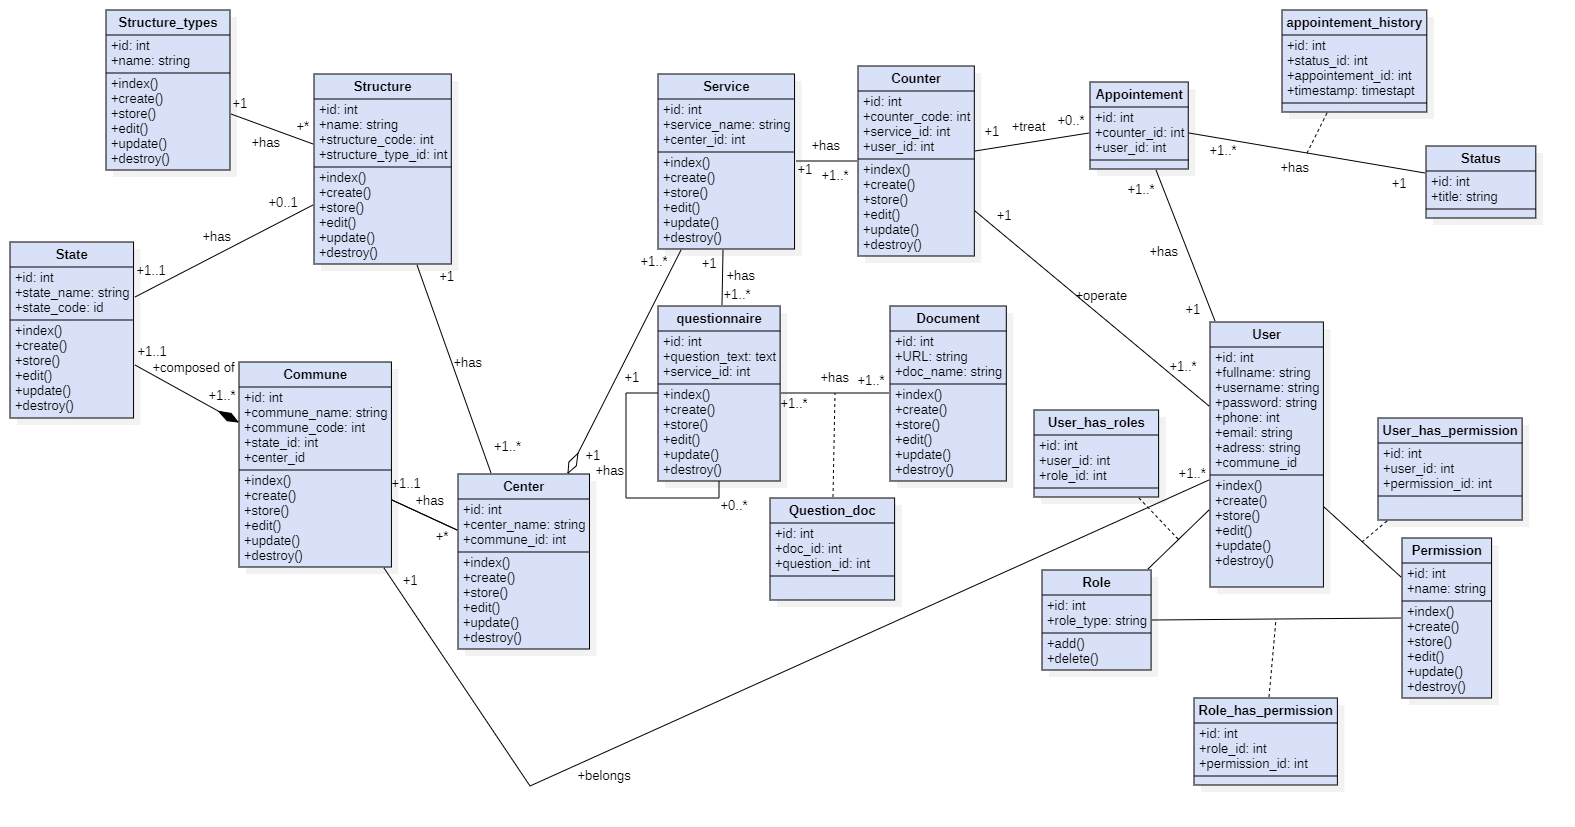
\includegraphics[width=1.1\textwidth]{ClassDiagram.png}
    \caption{Class diagram}
    \label{classdiagram}
\end{figure}
\newpage

\subsection{Discussion of the design decisions made}
Overall, the decision discussions we had during the process of elaborating the UML diagrams helped us to refine the system's design and functionality and to ensure that it met the requirements and expectations of both the users and the organization. The final UML diagrams illustrate the system's architecture and behavior in a clear and concise manner, and provide a solid foundation for building a robust and efficient virtual counter system for CNAS.

\medskip We came to a final conception of the virtual counter on the basis of the notion of eliminating the waiting time in such an effective way and to ensure an efficient system, which can provide by far a great user experience and a sturdy system. 
\newpage
\section{Database design}
At this juncture of conception, our primary focus was on creating a reliable database because a well-designed database is crucial for the efficient functioning of any application, including the virtual counter. We also made sure that accessing the data would be a secure process while also allowing stakeholders to track and store their data effectively.

\subsection{Overview of the database schema}
\begin{figure}[H]
    \centering
    \includegraphics*[width=0.3\textwidth]{SCREENSHOTS/overall.png}
    \caption{Overall Database Schema}
    \label{fig:overall-database-schema}
\end{figure}

\begin{figure}[H]
    \centering
    \includegraphics*[width=0.5\textwidth]{SCREENSHOTS/states.png}
    \caption{States Table}
    \label{fig:states-table}
\end{figure}

\begin{figure}[H]
    \centering
    \includegraphics*[width=0.5\textwidth]{SCREENSHOTS/structures.png}
    \caption{Structures Table}
    \label{fig:structures-table}
\end{figure}

\begin{figure}[H]
    \centering
    \includegraphics*[width=0.5\textwidth]{SCREENSHOTS/structuretypes.png}
    \caption{Structure Types Table}
    \label{fig:structures-types-table}
\end{figure}

\subsection{Discussion of the design decisions made}

The database for our web application consists of 16 tables, which are designed to store information related to states, communes, structures, structure\_types, services, users, roles, user\_has\_roles, permissions, role\_has\_permissions, appointments, questions, documents, questions\_documents, and user\_has\_permissions.

The decision to include these tables was  based on the needs of our application and the data that needs to be stored and managed. For example, tables such as states and communes are  included to help with location-based searches or queries, while tables like users and roles are necessary for managing user access and permissions.

The decision to use separate tables for each type of data is a common approach in database design, as it helps to organize the data and makes it easier to manage and query.

Overall, the decisions made regarding the database design for our web application are  based on the specific needs and requirements of our application, as well as best practices in database design and management. By carefully considering the data that needs to be stored and how it will be managed, you can ensure that our web application is efficient, scalable, and capable of delivering the functionality that our users need.